% Background chapter continued..

\section{Similarity Methods}
There are several methods available to calculate similarity score.
\\

\subsection{Cosine Similarity}
\label{cosine_similarity}
In this method \cite{19}, the result is the cosine of the angle between two vectors. Either between two item vectors or two profile vectors or one profile vector and item vector. The item ratings or preferences are stored in one vector called as item vector. The preferences of user are stored in another vector based on user's ratings and likes-dislikes is known as profile vector. Consider A and B are profile vector and item vector respectively, the similarity between them can be calculated as shown in \autoref{eq:cosine_similarity}.
\\

\begin{equation}
sim(A,B) = cos(\theta) =\frac {A.B}{\parallel A \parallel \parallel B \parallel}
\label{eq:cosine_similarity}
\end{equation}

\begin{figure}[H]
	\centering
	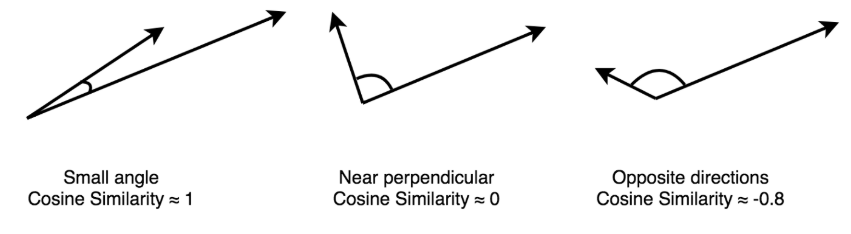
\includegraphics[width=0.7\linewidth]{cosine_similarity}
	\caption{Cosine Similarity}
	\label{fig:cosine_similarity}
\end{figure}

\noindent The value of cosine angle ranges between -1 to 1. Calculated result 0 shows that there is no similarity between vectors contrary to the result towards 1, which shows exact more similarity between vectors. As we can see in \autoref{fig:cosine_similarity} lesser the angle, less distance between vectors hence more similarity. Then items are arranged in descending order of similarity score and recommended to user.
\\
\subsection{Euclidean Distance Similarity}
\label{euclidean_distance}
The Euclidean distance between two points is the length which is connecting those two points. If we plot n dimensional space and plot similar items, then they will fall under close proximity. Consider example of positive quadrant of space and we plot items on the axis which are rated by user. The points drawn on graph represents score given by the user to those particular items. For more clear picture of this idea consider figure given below...
--- TO DO ----

 In that case, we can calculate distance between items with Euclidean distance formula which is given by:
\\
\begin{equation}
Euclidean Distance = \sqrt{(x_1 - y_1)^2 + ... + (x_n - y_n)^2}
\end{equation}


\subsection{Pearson's Correlation Similarity}
\label{pearson_correlation}
Person's correlation helps in finding correlation between two users or items. Correlation values ranges from -1 to 1 \cite{20}. Correlation on higher side implies more similarity. \autoref{eq:pearson_corr} gives correlation between two users $r_{u}$ and $r_{v}$.

\begin{equation}
sim(u,v) = \frac{\sum (r_{ui} - \bar{r}_u) (r_{vi} - \bar{r}_v )}{\sqrt{(\sum (r_{ui} - \bar{r}_u))^2} \sqrt{(\sum (r_{vi} - \bar{r}_v )^2}}
\label{eq:pearson_corr}
\end{equation}

Where $r_{ui}$ and $r_{vi}$ are rating scores for from two users. $\bar{r_{u}}$ and $\bar{r_{v}}$ denote the average rating by the two users.
Pearson correlation score $> 0$ indicates positive association. On the other hand, Pearson correlation score $ < 0$ indicates the negative correlation and score $ = 0$ indicates that no correlation. Hence correlation value can capture the rating similarity between two users. But if there are no common items between users that they have rated then the similarity measure will be considered as NAN results.
